% *******************************************************
% SUPPRESS WARNINGS
% *******************************************************
\RequirePackage{silence}
\WarningFilter{scrbook}{Usage of package `titlesec'}
\WarningFilter{titlesec}{Non standard sectioning command detected}

% *******************************************************
% DOCUMENT FRONT MATTER START
% *******************************************************
\documentclass[11pt,twoside,openright,titlepage,
  headinclude,footinclude,BCOR=5mm,
  numbers=noenddot,cleardoublepage=empty,
  tablecaptionabove, dottedtoc,
  bibliography=totoc]{scrreprt}
\usepackage{subfig}
\usepackage[eulerchapternumbers, subfig, beramono, eulermath, pdfspacing]{classicthesis} 
\usepackage{arsclassica}
\usepackage{amsmath}
\usepackage{amssymb}
\usepackage{graphicx}
\usepackage{booktabs}
\usepackage[utf8]{inputenc}
\usepackage[T1]{fontenc}
\usepackage{pdfpages}
\usepackage{titlesec}
\usepackage{titletoc}
\usepackage[norsk,american]{babel}
\usepackage[paperwidth=17cm, paperheight=24cm, margin=2.5cm]{geometry}
\usepackage[cam,a4,center,pdflatex]{crop}

% *******************************************************
% ADDITIONAL PACKAGES
% *******************************************************

% *******************************************************
% REFERENCE PACKAGES
% *******************************************************
  \usepackage[authoryear]{natbib}
  \bibliographystyle{plainnat}

% *******************************************************
% DEFINE VARIABLES
% *******************************************************
\newcommand{\Name}{Raju Rimal}
\newcommand{\Title}{Exploration of Multi-Response Multivariate Methods}
\newcommand{\Location}{\spacedlowsmallcaps{Ås}}
\newcommand{\Year}{2019}
\newcommand{\Month}{Jul}
\newcommand{\Date}{\Year, \Month}
\newcommand{\docsite}{\url{https://therimalaya.github.com/thesis}}
\newcommand{\Subtitle}{}
\newcommand{\email}{\mail{raju.rimal@nmbu.no}}
\newcommand{\homepage}{\url{https://www.mathatistics.com/}}
\newcommand{\Affiliation}{Biostatistics\\
Dept. of Chemistry, Biotechnology and Food Science\\
Norwegian University of Life Sciences}
\newcommand{\Faculty}{}
\newcommand{\Group}{}
\newcommand{\alttitle}{Utforskning av multi-respons multivariate metoder}

% *******************************************************
% CUSTOMIZATIONS
% *******************************************************
\newcommand{\mail}[1]{\href{mailto:#1}{\texttt{#1}}}
\titlecontents{part}[0pt]{\pagebreak}{}{\Large\MakeTextUppercase}{}
\titleformat{\part}[display]
  {\normalfont\centering\Large}%
  {\thispagestyle{empty}\partname~\MakeTextUppercase{\thepart}}{1em}%
  {\color{Maroon}\spacedallcaps}
\providecommand{\tightlist}{%
  \setlength{\itemsep}{0pt}\setlength{\parskip}{0pt}}
\DeclareTOCStyleEntry[beforeskip=3pt]{tocline}{section}

% *******************************************************
% DOCUMENT BEGIN
% *******************************************************
\begin{document}
\pagenumbering{Roman}
\pagestyle{plain}

% *******************************************************
% Title Front
% *******************************************************
\begin{titlepage}
  \pdfbookmark{Titlepage}{Titlepage}
  \begin{center}
    \large \sffamily
    \bigskip
    {\huge\spacedlowsmallcaps{\Title} \\}
    \bigskip
    {\large{\alttitle}} \\
    \vfill
    {\Large\spacedlowsmallcaps{Doctor of Philosophy (PHD) Thesis}} \\
    \bigskip
    {\Large{\spacedlowsmallcaps\Name}} \\
    \vfill
    {\normalsize \Affiliation}
    \vfill
    {\normalsize \Location, \Year \\}
    \vfill
              \newcommand{\logowidth}{0.6\linewidth}
          
\includegraphics[width=\logowidth]{Logo.pdf} \\
        \vfill
    {\normalsize
      Thesis Number: 1234:56\\
      ISSN:  1234-5678\\
      ISBN:  123-45-678-1234-5\\
    }
  \end{center}
\end{titlepage}

% *******************************************************
% Title Back
% *******************************************************
\thispagestyle{empty}
\hfill \vfill
\noindent
\textit{The goal is to turn data into information, and information into insight.}\\
\spacedlowsmallcaps{- Carly Fiorina, former CEO of Hewlett-Packard}
\vfill
\noindent
{\textbf{Supervisors:}} \\
Professor \textit{Solve Sæbø}\\
Prorector\\
Norwegian University of Life Sciences\\
Ås, Norway\\
\medskip\\
Associate Professor \textit{Trygve Almøy}\\
Dept. of Chemistry, Biotechnology and Food Science\\
Norwegian University of Life Sciences\\
Ås, Norway\\
\medskip\\
\bigskip \\
\noindent
\textit{\Title} \\
{\spacedlowsmallcaps{PhD Thesis, \Date\,\, \textcopyright\, \Name}} \\
\bigskip \\
\noindent{\spacedlowsmallcaps{Website}}: \\
\docsite \\
\medskip
\noindent{\spacedlowsmallcaps{E-mail}}: \\
\email
\vspace{1cm}
\hrule
\bigskip
\noindent This thesis is prepared with \texttt{ArsClassica} {\LaTeX} template with \texttt{pandoc} and r-package \texttt{bookdown}.
% \begin{flushright}source: \url{https://therimalaya.github.com/thesis}\end{flushright}
\pagestyle{scrheadings} 

% *******************************************************
% ABSTRACT
% *******************************************************

% *******************************************************
% SUMMARY
% *******************************************************
\begingroup
\pdfbookmark{Summary}{Summary}
\addchap{Summary}
A linear regression model defines a linear relationship between two or
more random variables. The random variables that depend on other random
variables are often called response variables and the independent random
variables are called predictor variables. In most cases not all
variation is relevant for regression, i.e.~only a certain amount of the
variation in the predictors is relevant and only so for a part of the
variation in the response. This leads to a reduction of the linear
regression model where one can imagine a subspace of the space spanned
by the predictor variables that contains all the relevant information
for a subspace of the space spanned by the response variables.

In this thesis we attempt to compare some new methods which are based on
the envelope model and some established methods such as principal
components regression (PCR) and partial least squares regression (PLS).
The comparison tests these methods on their performance of producing
minimum prediction and estimation error while modelling data simulated
with specifically designed properties. For the simulation we have also
created an R-package called \texttt{simrel} with a web interface.

A simulation model for a multi-response multivariate linear model, on
which the simulation tool is based, is discussed in the first paper.
This paper prepares a basic foundation for the simulations with the
concept of reduction of regression models. The second paper discusses
the similarities of the envelope, PCR and PLS population models. This
paper compares the prediction performance of several multivariate
methods using a model with a single response.

The final two papers make an extensive investigation evaluating the
prediction and estimation performance of established (PCR, PLS1 and
PLS2) and newly developed envelope based (Xenv and Senv) methods.
Unsurprisingly the study found that not one method dominates in all
situations, but their performance depend on the properties of the data
they model. However, the envelope based methods have shown remarkable
performance in many cases, both in prediction and estimation. The study
also recommend researchers to use and evaluate the envelope methods.


\KOMAoptions{open=left}
\begin{otherlanguage}{norsk}
\pdfbookmark{Sammendrag}{Sammendrag}
\addchap{Sammendrag}
En lineær regresjonsmodell definerer et lineært forhold mellom to eller
flere tilfeldige variabler. De tilfeldige variablene som er avhengige av
andre tilfeldige variabler kalles ofte responsvariabler og de uavhengige
tilfeldige variablene kalles prediktorvariabler. I de fleste tilfeller
er ikke alle variasjoner relevante for regresjon, dvs. bare en viss
mengde variasjoner i prediktorer er relevante for en del av variasjoner
i respons. Dette fører til en reduksjon av den lineære
regresjonsmodellen der man kan forestille seg et underområde av plassen
som spennes av prediktorvariablene som inneholder all relevant
informasjon for et underområde spandert av responsvariablene.

I denne avhandlingen prøver vi å sammenligne noen nye metoder som er
basert på konvoluttmodellen og noen etablerte metoder som
hovedkomponenter regresjon (PCR) og partiell minste kvadraters regresjon
(PLS). Sammenligningen tester disse metodene på deres ytelse til å
produsere minimum prediksjon og estimeringsfeil mens modelleringsdata
simuleres med spesielt designet egenskaper. For simuleringen har vi også
laget en R-pakke kalt \texttt{simrel} med et webgrensesnitt.

En første simuleringsmodell for en multirespons, multivariat lineær
modell som simuleringsverktøyet bygger på. Denne artikkelen utarbeider
et grunnleggende fundament for simuleringene med konseptet reduksjon av
regresjonsmodeller. Den andre artikkelen diskuterer likhetene i
konvolutt-, PCR- og PLS-populasjonsmodellene. Denne artikkelen
sammenligner prediksjonsytelsen til flere multivariate metoder ved bruk
av en modell med en enkelt respons.

\end{otherlanguage}{norsk}
\KOMAoptions{open=right}
\endgroup

% *******************************************************
% ACKNOWLEDGMENT
% *******************************************************
\pdfbookmark{Acknowledgments}{Acknowledgments}
\begingroup
\cleardoublepage
\addchap{Acknowledgment}
\input{chapters/00-Acknowledgment.md}
\endgroup

% *******************************************************
% PREFACE
% *******************************************************
\pdfbookmark{Preface}{Preface}
\begingroup
\cleardoublepage
\addchap{Preface}
This thesis is a part of Doctor of Philosophy (PhD) study. The first
part of the thesis constitute of a gentle introduction to the objective
of the study and some of its background. This is followed by the summary
of individual research paper on which this thesis is based on. The
discussion section tries to bind the finding from theses papers. The
final chapter will discuss the limitations and future prospect of the
study. The second part contains all the papers attached.

An R-package called \texttt{simrel} is available as part of the first
paper included in this thesis. The package lets users to simulated data
from multi-response linear model. The package can be install from
R-package repository CRAN or from GitHub
(\url{https://github.com/simulatr/simrel}). In addition, a web
application that gives users a graphical user interface for the package
is also available from GitHub. All the results and the documentations of
the research can be reproduced from the codes in GitHub repository with
softwares and packages required are installed. In addition, one can use
docker image together with the code for reproducing the thesis together
with all included papers. All related resources are list in the final
chapter.

\endgroup

% *******************************************************
% INCLUDE ANYTHING BEFORE
% *******************************************************

% *******************************************************
% Contents
% *******************************************************
\cleardoublepage
\phantomsection
\pdfbookmark{\contentsname}{tableofcontents}
\setcounter{tocdepth}{2}
\begingroup 
  \let\clearpage\relax
  \let\cleardoublepage\relax
    \tableofcontents
\endgroup
\markboth{\spacedlowsmallcaps{\contentsname}}
{\spacedlowsmallcaps{\contentsname}} 

\begingroup
\cleardoublepage
\listoftables
\vfill
\let\clearpage\relax
\let\cleardoublepage\relax

\listoffigures
\vfill
\endgroup

\begingroup 
  \let\clearpage\relax
  \let\cleardoublepage\relax
\endgroup

\cleardoublepage

% *******************************************************
% BODY START
% *******************************************************

\pagenumbering{arabic}

\hypertarget{introduction}{%
\chapter{Introduction}\label{introduction}}

As a consequence of the development in the technology and computing power, data science discipline has emerged from the explosion of data. Extracting information from this chaotic heap of data has become another problem. Many statistical and machine learning tools are being devised for this purpose. However the difference in the approach, these methods target the problem, makes them distinct and useful to deal with certain aspect of the data. Most of these problems lie in identifying the relationship between variables. This thesis confined itself in the exploration of linear relationship where a set of independent variables called predictor variables affect another set of dependent variables called response variables. Normally only subspace of predictor variables are relevant for a subspace of response variables to define its linear relationship. This brings to the concept of relevant and irrelevant space. Methods like Principal Components Regression (PCR), Partial Least Squares (PLS) and many other variants of PLS has leveraged this concept and are serving as a prime tool in many discipline, most notably chemometrics. A relatively new methods called envelopes has used this concept of dimension reduction such that only the relevant (material) part in both response and predictors can be used to estimate the underlying linear model. Although the underlying population model is similar in these methods, they estimate the model parameter differently. Evaluation of these methods is crucial in order to understand their pros and cons on dataset with certain properties. This thesis will explore some of these methods and access their estimative and predictive strength and weaknesses through both simulated and real datasets. This exploration adds a reference for researchers and motivates them for using different methods based on the properties of the data they are working on.

This study is exploratory in nature where we assess and compare different multi-response multivariate methods but most importantly study their interaction with the properties of the data. The properties include the correlation between predictor variables, the position of principal components of predictor variables (predictor components) that are relevant for certain principal components of response variables (response components), the amount of correlation between the response variables and the number of predictor variables. The effect of correlation structure of response matrix is less explored and it is expected to add some light on how similar and how different the methods are in terms of modelling this structure. In order to simulate data with these properties varying at different levels, we have created an R-package called \texttt{simrel} which is an extension of the previous version of it introduced by \citet{saebo2015simrel} to incorporate multiple response.

\hypertarget{background}{%
\chapter{Background}\label{background}}

Following subsections will discuss few related topics extensively used in the papers.

\hypertarget{multivariate-linear-regression-model}{%
\section{Multivariate Linear Regression Model}\label{multivariate-linear-regression-model}}

We can write the joint distribution of a random variable \(\mathbf{y}\) consists of \(m\) response variables and another random variable \(\mathbf{x}\) consists of \(p\) predictor variables as,

\begin{equation}
\begin{bmatrix}
  \mathbf{y}\\
  \mathbf{x}
\end{bmatrix} \sim
\mathsf{N}\begin{pmatrix}
  \begin{bmatrix}
    \boldsymbol{\mu_y}\\
    \boldsymbol{\mu_x}
  \end{bmatrix},
  \begin{bmatrix}
    \boldsymbol{\Sigma_{yy}} &
    \boldsymbol{\Sigma_{yx}} \\
    \boldsymbol{\Sigma_{xy}} &
    \boldsymbol{\Sigma_{xx}}
  \end{bmatrix}
\end{pmatrix}
\label{eq:linear-model}
\end{equation}

A model that linearly relates \(\mathbf{x}\) and \(\mathbf{y}\) through regression coefficient \(\boldsymbol{\beta}\) is often written as,

\begin{equation}
\mathbf{y} = \boldsymbol{\mu}_y + \boldsymbol{\beta}^t\left(\mathbf{x} - \boldsymbol{\mu}_x\right) + \boldsymbol{\varepsilon}
\label{eq:linear-reg-model}
\end{equation}
where \(\boldsymbol{\varepsilon} \sim \textsf{N}\left(\mathbf{0}, \boldsymbol{\Sigma}_{y|x}\right)\), \(\boldsymbol{\mu}_y\) is the mean vector of \(\mathbf{y}\) and \(\boldsymbol{\mu}_x\) is the mean vector of \(\mathbf{x}\).

We can write the regression coefficient \(\boldsymbol{\beta} = \boldsymbol{\Sigma}_{xx}^{-1}\boldsymbol{\Sigma}_{xy}\) in terms of the covariance matrices. A complete simulation of this model requires to identify \(1/2(p+m)(p+m+1)\) unknowns. However, not all information in \(\mathbf{x}\) are relevant for \(\mathbf{y}\) and not everything in \(\mathbf{y}\) are informative. We can refer the space with information as relevant (informative) space and the rest as irrelevant (uninformative) space. \citet{saebo2015simrel} and \citet{Rimal2018} have parameterized the linear model \eqref{eq:linear-model} based on the concept of relevant space and provided a tool for simulating multi-response data with few tuning parameters. A review on the simulation and the experimental design adopted in various papers attached to this thesis will follow after a short discussion of relevance and irrelevance in linear model.

\hypertarget{relevant-space-and-relevant-components}{%
\section{Relevant Space and Relevant Components}\label{relevant-space-and-relevant-components}}

\citet{Naes1985} introduced the definition of relevant space as the decomposition of predictor space into two orthogonal subspaces: relevant and irrelevant such that a set of latent components defined as irrelevant components have no correlation with the response and no correlation with the relevant part of the data. The concept was further discussed and developed by \citet{helland1990partial} and \citet{naes1993relevant}. More recently, various estimators \citep{cook2010envelope, cook2013envelopes, cook2015simultaneous} based on envelope \citep{Cook2007a} have used the concepts of separation of relevant and irrelevant spaces which they have referred as material and immaterial spaces.

\begin{figure}[!htb]
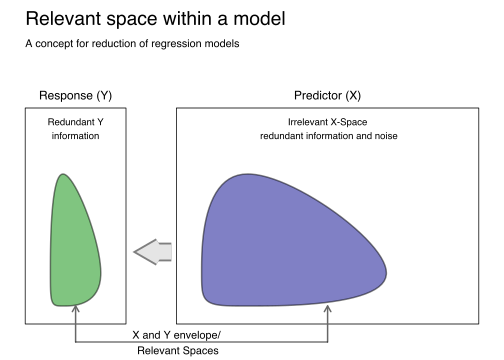
\includegraphics[width=1\linewidth]{Thesis_files/figure-latex/relspace-plot-1} \caption{Relevant and Irrelevant Space in Linear Model}\label{fig:relspace-plot}
\end{figure}

The concept can also be extended to the response such that a subspace contains the information relevant for a model that the relevant space in \(\mathbf{x}\) can explain. The item is implemented in simulteneous envelope \citep{cook2015simultaneous} and response envelope \citep{cook2010envelope} methods. However methods such as PCR and PLS1 have not used the reduced space in the response. Figure-\ref{fig:relspace-plot} shows the notion of this reduction of linear regression model.

\hypertarget{simulation}{%
\section{Simulation}\label{simulation}}

Simulation refers to generate the data from known underlying population structure. Controlling the properties of the population is vital in the simulation which enables researchers and users to use the data for comparison of methods, accessing new methodology, testing theory and evaluating alorithms. Such data can also be widely used for educational purposes. All the research studies in this thesis have used an R-package called \texttt{simrel} for simulating multi-response linear model data introduced by \citet{RIMAL20181}. The simulation tool is general purpose in nature and has few parameters that controls the essential properties of the poulation enabling users to simulate data with wide range of properties.

The population properties such as the coefficient of determination, number of relevant predictors, level of multicollinerity and the position of relevant principal components can be varied in the simulation with \texttt{simrel}. A full factorial experimental design on various levels of some of these population properties has been implimented in all of these studies for various comparison. An experimental design helps to analyse the effect of certain population properties and allows comparision of different levels of these factors and their interactions. The data obtained from the simulation are used to compare different methods based on their performance. The performance is accessed through there prediction and estimation ability.

\hypertarget{estimation-and-prediction}{%
\section{Estimation and Prediction}\label{estimation-and-prediction}}

Measures such as mean and standard deviation for a population are usually referred as parameters of the population. A model as in \eqref{eq:linear-reg-model}, which tries to formulate the relationship between \(\mathbf{x}\) and \(\mathbf{y}\) in the population uses parameters such as the error variance and regression coefficients are also terms as parameters. Usually, due to the lack of known population distribution, the values of these parameters are calculated using a sample collected from that population. The process of determining the value of certain parameters is called estimation. The estimated value from any two samples are different. The estimated values are considered better if squared difference between the estimated and true value is small and have small variation. The goodness of the estimates depends on the nature of the data and the method that is used to estimate them. In estimation error for a certain method using the simulated data with specific properties in most of the comparisons in this thesis are computed as in \eqref{eq:est-error}.

\begin{equation}
\text{Estimation Error} = \mathsf{E}\left[
  \left(\boldsymbol{\beta} - \hat{\boldsymbol{\beta}}\right)^t 
  \left(\boldsymbol{\beta} - \hat{\boldsymbol{\beta}}\right)
\right]
\label{eq:est-error}
\end{equation}

A fitted or trained model are mostly used for prediction. Prediction referes to determining the value of the response for a new set of predictor which were not used to train the model. Most studies under ``data science'' field are targeted for better prediction. Most comparison in this thesis evaluate the prediction performance of the multivariate methods using the prediction error measured as in \eqref{eq:pred-error}.

\begin{equation}
\text{Prediction Error} = \mathsf{E}\left[
  \left(\boldsymbol{\beta} - \hat{\boldsymbol{\beta}}\right)^t
  \boldsymbol{\Sigma}_{xx}
  \left(\boldsymbol{\beta} - \hat{\boldsymbol{\beta}}\right)
\right] + \boldsymbol{\Sigma}_{y|x}
\label{eq:pred-error}
\end{equation}

\begin{itemize}
\tightlist
\item
  Prediction error are influenced by the covariance of the predictor directly while estimation error are not
\item
  In the case of multicollinear predictors, estimation error can be huge while due to the scaling of the covariation of predictors, the prediction error can still be small
\item
  A good estimation can give proper and trustworthy idea about the relation between certain predictor variation with certain response variable
\item
  This is important in policy making, academic researches and to understanding the relation to develope new models.
\item
  Prediction on the other hand are widely used from weather forcasting, economic forecasting, prediction in production and sales and many more.
\end{itemize}

\hypertarget{multivariate-methods}{%
\section{Multivariate Methods}\label{multivariate-methods}}

Various multivariate methods such as ordinary least squares (OLS), principal components regression (PCR), partial least squares (PLS) regression and envelope methods are used for comparison of the study included in this thesis. All of these methods except OLS use the concept of relevant space and the reduction of the regression model.

\citet{WENTZELL2003257} has assmbled many comparisons made on PCR and PLS where they conclude that PLS have not shown clear advantage over PCR over predictive ability in most studies but uses less number of components than PCR. As PLS has been both popular and productive in fields like chemometrics, its developement has progressed quickly over time throught the formulation of various derivetives. CPLS and CPPLS are among them which conbines PLS and cannonical correlation analysis (CCA) and gives a joint framework for classification and regression \citep{indahl2009canonical}. The first included paper which has introduced the simulation tool \texttt{simrel} has made some basic comparison on these methods for their predictive ability. The third and fourth paper included have made elaborative comparison on PCR and PLS using various properties in the data. More discussion are in the summary section of the respective papers. In addition, PLS1 methods which models each response separatly without any knowledge of other responses are also included. Further, in the single response setting, the second paper includes BayesPLS \citep{helland2012near} method in the comparison which have shown promishing results.

Many literature are available comparing PCR, PLS and their derivetive. However there are not any studies to date which have made any emperical comparisons of newly developed \emph{envelope} based methods using real and simulated data with these more established methods. Envelope introduced by \citet{Cook2007a} have been used to develop various estimators including response envelope (Yenv), predictor envelope (Xenv) and simultaneous estimation of envelope in both predictor and response (Senv). Envelope is defined as the smallest subspace that includes the span of true regression coefficients. The comparisons of these envelope methods together with PCR and PLS in third and fourth paper has shown encouraging results for envelope methdods in both easy and difficult models.

Details on each of these methods can be obtained from the corresponding references.

\hypertarget{experimental-design}{%
\section{Experimental Design}\label{experimental-design}}

In all the comparison, different simulation parameters are considered as factors and the prediction and estimation error are considered as outcome variables. Factorial Design are implemented as an experimental design which allowed us to compare all possible combination of different factor levels. For Example, the factorial design used throughout the third and fourth paper shown in Figure \ref{fig:design-plot} has four factors: Number of predictor variables (\texttt{p}) with two levels, level of multicollinearity (\texttt{gamma}) with two levels where higher value represents higher level of multicollinearity, position index of relevant predictor components (\texttt{relpos}) and the level of collinearity in response (\texttt{eta}) with four levels where higher value represents higher correlation between the response variables. The combination of these factors have created 32 unique designs which are then used for simulating data with that particular properties. Such data, with all possible combination of these properties, have made both through and regorous comparison of the methods fisible.



\begin{figure}[!htb]
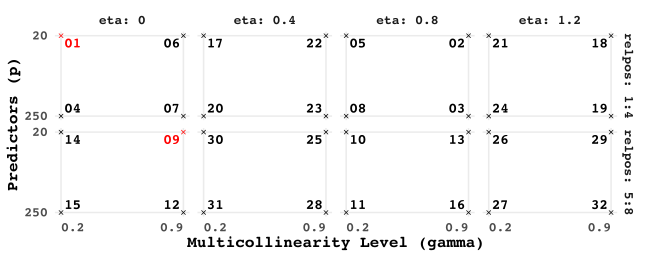
\includegraphics[width=1\linewidth]{Thesis_files/figure-latex/design-plot-1} \caption{An example of factorial design used in the third and fourth paper.}\label{fig:design-plot}
\end{figure}

Lets dig a little deeper to understand how these simulation parameters are tied with the properties of the simulated data. As an example, let us take Design 1 and Design 9 of Figure \ref{fig:design-plot} where data simulated with Design 1 have low multicollinearity and the position index of relevant predictors are at 1, 2, 3, 4 while Design 9 have high multicollinearity and the position index of relevant predictors are at 5, 6, 7, 8. All the other factors or properties of the data being same for both, the difference is these two design helps us to analyse the interaction between the multicollinearity in the data and the position of relevant components.



\begin{figure}[!htb]
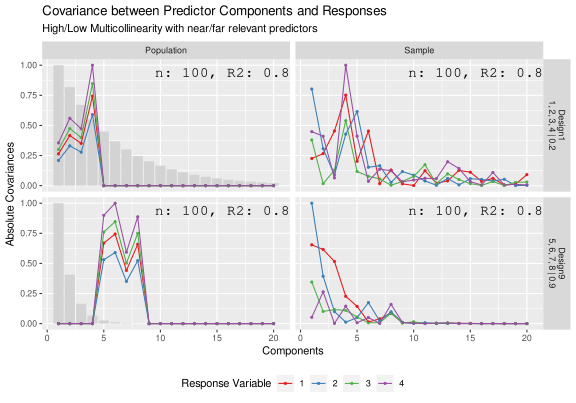
\includegraphics[width=1\linewidth]{Thesis_files/figure-latex/cov-plot-1} \caption{\emph{Design 1}: Relevant components have large variation, \emph{Design 9}: irrelevant components have large variation and relevant components have small variation.}\label{fig:cov-plot}
\end{figure}

Figure \ref{fig:cov-plot} (top-row) shows the scaled covariance between the predictor components and the response variables for Design 1. Here the relevant components with larger variation (due to low multicollinearity) simulates data that are easier to model my most methods. Figure \ref{fig:cov-plot} (bottom-row) for Design 9 shows that the relevant components at position 5, 6, 7, 8 has small variation and irrelevant components at position 1, 2, 3, 4 have large variation. This design simulates data that are difficult to model my most methdos. The population covariances in the figure gives clear and distinct relationship while the sample covariances have somewhat rough approximation of the population.

\hypertarget{analysis-of-variance}{%
\section{Analysis of Variance}\label{analysis-of-variance}}

Performance measures such as prediction error, estimation error and the number of components used by the methods under comparison, various plots together with principal components analysis (PCA) has been used. In addition, a more formal analysis is made using analysis of variance (ANOVA). ANOVA allowed us not only to understand the effect of various properties of data controlled by the simulation parameters but also analysis the effect of interaction of these properties with the methods. Third and fourth paper with four response variables each of which are analyzed together with multivariate analysis of variance (MANOVA).

Multivariate analysis of variance (MANOVA) is the multivariate counterpart of the ANOVA where various test statistic is used such as Wilks' Lambda, Lawley-Hotelling trace, Pillai trace and Roy's largest root. All of these methods use the within \((\mathbf{E})\) and between \((\mathbf{H})\) sum of squares and the cross products matrix. All four test statistic are nearly equivalent for large sample size \citep{johnson2018applied}. In our studies, Pillai trace is used which is defined as,

\begin{equation}
\text{Pillai statistic} = \text{tr}\left[(E + H)^{-1}H\right] = \sum_{i=1}^{m}{\frac{\nu_i}{1+\nu_i}}
\label{eq:pillai}
\end{equation}
where, \(\nu_i\) represents the eigenvalues corresponding to \(\mathbf{E^{-1}H}\).

\hypertarget{paper-summary}{%
\chapter{Paper Summary}\label{paper-summary}}

\hypertarget{paper-1-a-tool-for-simulating-multi-response-linear-model-data}{%
\section{Paper 1: A tool for simulating multi-response linear model data}\label{paper-1-a-tool-for-simulating-multi-response-linear-model-data}}

\begin{itemize}
\tightlist
\item
  Extend the simulation tool introduced by \ldots solve2015simrel\ldots{} for multi-response simulation
\item
  Gives the mathematical formulation for the simulation
\item
  Makes basic comparison on various multivariate methods using both simulated and real data
\item
  Shows that \ldots{}
\end{itemize}

\hypertarget{paper-2-model-and-estimators-for-partial-least-squares-regression}{%
\section{Paper 2: Model and estimators for partial least squares regression}\label{paper-2-model-and-estimators-for-partial-least-squares-regression}}

\begin{itemize}
\tightlist
\item
  The paper shows the similarity of population model of PCR, PLS and envelope in predictors
\item
  My contribution on the paper is on the example of a comparative study with single response with both simulated and real data
\item
  BayesPLS showed better performance with few fallback such as crashing, time consuming and lack of method for multi-response model
\item
  It also showed that \ldots{} on the prediction performance
\end{itemize}

\hypertarget{paper-3-comparison-of-multi-response-prediction-methods}{%
\section{Paper 3: Comparison of Multi-response Prediction Methods}\label{paper-3-comparison-of-multi-response-prediction-methods}}

\begin{itemize}
\tightlist
\item
  This paper extends the comparative study on both of the previous paper
\item
  Here only methods based on relevant space is considered for comparison
\item
  A small modification in the envelope methods is made as the methods is based on maximum likelihood and can not be fitted on \(p>>n\) case.
\item
  The results showed that \ldots{}
\end{itemize}

\hypertarget{paper-4-comparison-of-multi-response-estimation-methods}{%
\section{Paper 4: Comparison of Multi-response Estimation Methods}\label{paper-4-comparison-of-multi-response-estimation-methods}}

\begin{itemize}
\tightlist
\item
  Since good prediction not always results in good estimation, this paper continue the exploration of Paper3 for the estimation performance of the methods
\item
  The same data is used with the similar modification in envelope methods
\item
  The interaction of methods and the design on the basis of error is studied with MANOVA in both Paper3 and Paper4
\end{itemize}

\hypertarget{discussions-conclusions-and-future-perspectives}{%
\chapter{Discussions, Conclusions and Future Perspectives}\label{discussions-conclusions-and-future-perspectives}}

\hypertarget{discussions-and-conclusions}{%
\section{Discussions and Conclusions}\label{discussions-and-conclusions}}

\begin{itemize}
\tightlist
\item
  Get the conclusion of all the papers
\item
  Add a paragraph to say something on big picture
\end{itemize}

\hypertarget{previous-studies}{%
\chapter{Previous Studies}\label{previous-studies}}

\begin{itemize}
\tightlist
\item
  Previous similar studies
\item
  Mostly used the methods developers
\item
  Connection with data properties in an experimental manner is not explored properly and comprehensively
\item
  Effect on multi-response model and the effect of correlation structure on the methods is not studied for these methods to our knowledge
\item
  Envelope model is not accessed in these applied setting and data related to chemometrics
  The exploration and findings of the papers are discussed in brief in next chapter.
\end{itemize}

\hypertarget{limitations-and-future-perspectives}{%
\section{Limitations and Future Perspectives}\label{limitations-and-future-perspectives}}

\begin{itemize}
\tightlist
\item
  Ridge, Lasso and other methods could have been used for comparison but since they are not based on the relevant components. Although we did some basic comparison by including them but they require a separate and comprehensive study.
\item
  Highly applied form of comparison but it can be extended also to the comparison of their mathematical formulation. This has been done in second paper for a single response case but the simultaneous envelope and multi-response case needs a separate study.
\item
  In the current state, the simulation tool assumes that the predictor components relevant for one response components is not relevant for another. This can be further studied and can be extended to simulate more general data structure.
\item
  The simulation tool can also be extended to simulate ANOVA model and model with multi-class categorical response model. This increases the applicability of tools in more research areas and educational purpose.
\end{itemize}

% *******************************************************
% BIBLIOGRAPHY START
% *******************************************************
  \renewcommand\bibname{References}
 % has-chapters
 % biblio-title
  \bibliography{References.bib}
 % bibliography
 % natbib

 % biblatex

\nocite{*}

% *******************************************************
% PAPER START
% *******************************************************
\appendix
\part*{List of Research Papers}
\par\chapter{A tool for simulating multi-response linear model data}
\cleardoublepage
\includepdf[pages=-1]{papers/001.pdf}
%\includepdf[pages=-]{papers/001.pdf}
\par\chapter{Model and estimators for partial least squares regression}
\cleardoublepage
\includepdf[pages=-1]{papers/002.pdf}
%\includepdf[pages=-]{papers/002.pdf}
\par\chapter{Comparison of Multi-response Prediction Methods}
\cleardoublepage
\includepdf[pages=-1]{papers/003.pdf}
%\includepdf[pages=-]{papers/003.pdf}
\par\chapter{Comparison of Multi-response Estimation Methods}
\cleardoublepage
\includepdf[pages=-1]{papers/004.pdf}
%\includepdf[pages=-]{papers/004.pdf}

% *******************************************************
% ANYTHING EXTRA
% *******************************************************

\end{document}

%%% Local Variables:
%%% mode: latex
%%% TeX-master: t
%%% End:
